\begin{name}
	{\tenchude}
	{TOÁN 12}
	{LỚP TOÁN THẦY PHÁT}
	{Thời gian: 90 phút - Không kể thời gian phát đề}
\end{name}
\Opensolutionfile{ans}[ans/ansDe4-TN1]
\begin{ex}%[2D4N1-1]%[2015_K12 Huyên Nguyễn]
	Cho $F(x)$ là nguyên hàm của hàm số $f(x)=\sin \left(\dfrac{\pi}{2}-x\right)$. Khi đó $F'(x)$ bằng
	\choice
	{$\cos \left(\dfrac{\pi}{2}-x\right)$}
	{$\sin x$}
	{$-\cos \left(\dfrac{\pi}{2}-x\right)$}
	{\True $\cos x$}
	\loigiai{
		Vì $F(x)$ là một nguyên hàm của hàm số $f(x)$ nên $F'(x)=f(x)=\sin \left(\dfrac{\pi}{2}-x\right)=\cos x$.
	}
\end{ex}

\begin{ex}%[2D4N1-2]%[2015_K12 Huyên Nguyễn]
	Cho $F(x)$ là một nguyên hàm của hàm số $f(x)=\dfrac{1}{x}$ và thỏa mãn $F\left(\mathrm{e}^2\right)=3$. Khi đó $F(x)$ bằng
	\choice
	{$\ln |x|+5$}
	{\True $\ln |x|+1$}
	{$\ln |x|+3$}
	{$\ln |x|-1$}
	\loigiai{
		Ta có $F(x)=\displaystyle\int\dfrac{1}{x}\mathrm{\,d}x=\ln |x|+C$.\\
		Mà $F\left(\mathrm{e}^2\right)=3\Leftrightarrow \ln |\mathrm{e}^2|+C=3\Leftrightarrow C=1$.\\
		Vậy $F(x)=\ln |x|+1$.
	}
\end{ex}

\begin{ex}%[2D4H1-3]
	Cho hàm số $f(x)=3\cos x-\dfrac{2}{x}+\dfrac{4}{{{\sin }^2}x}$. Khẳng định nào dưới đây là đúng?
	\choice
	{\True $\displaystyle\int{f(x)\mathrm{d}x}=3\sin x-2\ln |x|-4\cot x+C$}
	{ $\displaystyle\int{f(x)\mathrm{d}x}=3\sin x-2\ln x-4\cot x+C$}
	{ $\displaystyle\int{f(x)\mathrm{d}x}=3\sin x-2\ln |x|+4\cot x+C$}
	{ $\displaystyle\int{f(x)\mathrm{d}x}=-3\sin x-2\ln |x|-4\cot x+C$}
	\loigiai{
		Ta có $\displaystyle\int{f(x)\mathrm{d}x}=\displaystyle\int{(3\cos x-\dfrac{2}{x}+\dfrac{4}{{\sin^2}x})\mathrm{d}x}$ \\
		$=3\displaystyle\int{\cos x\mathrm{d}x}-2\displaystyle\int{\dfrac{1}{x}\mathrm{d}x}+4\displaystyle\int{\dfrac{1}{{\sin^2}x}\mathrm{d}x}$ \\
		$=3\sin x-2\ln |x|-4\cot x+C$.
	}
\end{ex}

\begin{ex}%[2D4H2-1]
	Biết $F(x)=x^2$ là một nguyên hàm của hàm số $f(x)$ trên $\mathbb{R}$. Giá trị của $\displaystyle  \int\limits_1^2\left[2+f(x)\right]\mathrm{\,d}x$ bằng
	\choice
	{$3$}
	{\True $5$}
	{$\dfrac{13}{3}$}
	{$\dfrac{7}{3}$}
	\loigiai{
		Ta có $\displaystyle  \int\limits_1^2\left[2+f(x)\right]\mathrm{\,d}x$ $=\left.(2x+x^2)\right|_1^2=8-3=5$.
	}
\end{ex}

\begin{ex}%[2D4N3-1]
	Gọi $S$ là diện tích hình phẳng giới hạn bởi các đường $y=3^x$, $y=0$, $x=0$ và $x=2$. Mệnh đề nào dưới đây là đúng?
	\choice
	{$S=\pi \displaystyle\int\limits_{0}^{2}{3^x}\mathrm{\,d}x$}
	{$S=\displaystyle\int\limits_{0}^{2}{3^{2x}}\mathrm{\,d}x$}
	{\True $S=\displaystyle\int\limits_{0}^{2}{3^x}\mathrm{\,d}x$}
	{$S=\pi \displaystyle\int\limits_{0}^{2}{3^{2x}}\mathrm{\,d}x$}
	\loigiai
	{Diện tích hình phẳng giới hạn bởi các đường $y=3^x$, $y=0$, $x=0$ và $x=2$ là $S=\displaystyle\int\limits_{0}^{2}{\left|3^x\right |}\mathrm{\,d}x = \displaystyle\int\limits_{0}^{2}{3^x}\mathrm{\,d}x$.}
\end{ex}

\begin{ex}%[Dự án 2025 - đề cấu trúc mới, Hung Doan]%[2D4H3-3]
	Tính thể tích khối tròn xoay được tạo bởi hình phẳng giới hạn bởi đồ thị hàm số $y=3x-x^2$ và trục hoành khi quay quanh trục hoành.
	\choice
	{$\dfrac{85\pi}{7}$}
	{$\dfrac{8\pi}{7}$}
	{\True $\dfrac{81\pi}{10}$}
	{$\dfrac{41\pi}{7}$}
	\loigiai{
		Phương trình hoành độ giao điểm của đồ thị hàm số $y=3x-x^2$ và trục hoành là \[3x-x^2=0\Leftrightarrow \hoac{&x=0\\&x=3.}\]
		Thể tích của khối tròn xoay là $V=\pi \displaystyle\int \limits_0^3 (3x-x^2)^2\mathrm{\,d}x=\dfrac{81\pi}{10}$.}
\end{ex}

\begin{ex}%[2H5N1-1]%[Dự án Khối 12- Ex-TF-TLN-2024]%[VU Ngoc Hao]
	\immini{
		Cho hình hộp chữ nhật $ABCD.A'B'C'D'$. Bốn véc-tơ pháp tuyến  của mặt phẳng $\left(AA'B'B\right)$ là
		\choice
		{$\overrightarrow{AD}$, $\overrightarrow{A'D'}$, $ \overrightarrow{BD}$, $\overrightarrow{B'C'}$}
		{$\overrightarrow{AD}$, $\overrightarrow{A'D'}$, $ \overrightarrow{BC}$, $\overrightarrow{BC'}$}
		{$\overrightarrow{AC}$, $\overrightarrow{A'D'}$, $ \overrightarrow{BC}$, $\overrightarrow{B'C'}$}
		{\True  $\overrightarrow{AD}$, $\overrightarrow{A'D'}$, $ \overrightarrow{BC}$, $\overrightarrow{B'C'}$}
	}
	{
		\begin{tikzpicture}[scale=0.5, font=\footnotesize,line join=round, line cap=round, >=stealth]
			\coordinate (A) at (0,0);
			\coordinate (B) at (-2,-1.5);
			\coordinate (D) at (5,0);
			\coordinate (C) at ($(B)+(D)-(A)$);
			\foreach \i in {A,B,C,D}{\coordinate (\i') at ($(\i)+(0,4)$);}
			\draw (A')--(B')--(C')--(D')--cycle;
			\draw (B)--(B') (C)--(C') (D)--(D')  (B)--(C)--(D);
			\draw[dashed,thin](B)--(A)--(A') (A)--(D);
			\foreach \i/\g in {A'/90,B'/90,C'/90,D'/90,A/-90,B/-90,C/-90,D/-90}{\draw[fill=black](\i) circle (1pt) ($(\i)+(\g:5mm)$) node[scale=1]{$\i$};}
		\end{tikzpicture}
	}
	\loigiai{
		Bốn véc-tơ pháp tuyến của mặt phẳng $\left(AA'B'B\right)$ là  $\overrightarrow{AD}$, $\overrightarrow{A'D'}$, $ \overrightarrow{BC}$, $\overrightarrow{B'C'}$.
	}
\end{ex}

\begin{ex}%[2H5N1-2]
	Trong không gian với hệ tọa độ $Oxyz$, cho mặt phẳng $(P)\colon x-y+3=0$. Véc-tơ nào sau đây \textbf{không phải} là véc-tơ pháp tuyến của mặt phẳng $(P)$?
	\choice
	{$\overrightarrow{a}=(3;-3;0)$}
	{\True $\overrightarrow{a}=(1;-1;3)$}
	{$\overrightarrow{a}=(1;-1;0)$}
	{$\overrightarrow{a}=(-1;1;0)$}
	\loigiai{
		Véc-tơ pháp tuyến của mặt phẳng $(P)$ là $\overrightarrow{n}=(1;-1;0)$.\\
		Ta có $\overrightarrow{a}=(-1;1;0)=-(1;-1;0)=-\overrightarrow{n}$. Vậy $\overrightarrow{a}=(-1;1;0)$ là một véc-tơ pháp tuyến của mặt phẳng $(P)$.\\
		Tương tự $\overrightarrow{a}=(3;-3;0)=3(1;-1;0)=3\overrightarrow{n}$. Vậy $\overrightarrow{a}=(3;-3;0)$ là một véc-tơ pháp tuyến của mặt phẳng $(P)$.\\
		Do véc-tơ $\overrightarrow{a}=(1;-1;3)$ không cùng phương với véc-tơ $\overrightarrow{n}=(1;-1;0)$. Nên $\overrightarrow{a}=(1;-1;3)$ không là véc-tơ pháp tuyến của mặt phẳng $(P)$.
	}
\end{ex}

\begin{ex}%[2H5H1-3]
	Trong không gian $O x y z$, phương trình của mặt phẳng $(P)$ đi qua điểm $B(2 ; 1 ;-3)$, đồng thời vuông góc với hai mặt phẳng $(Q)\colon x+y+3 z=0,$ $(R)\colon 2 x-y+z=0$ là
	\choice
	{$4 x+5 y-3 z+22=0$}
	{$4 x-5 y-3 z-12=0$}
	{$2 x+y-3 z-14=0$}
	{\True $4 x+5 y-3 z-22=0$}
	\loigiai{
		Mặt phẳng $(Q)\colon x+y+3 z=0,$ $(R)\colon 2 x-y+z=0$ có các véc-tơ pháp tuyến lần lượt là $\overrightarrow{n}_1=(1 ; 1 ; 3)$ và $\overrightarrow{n}_2=(2 ;-1 ; 1)$.\\
		Vì $(P)$ vuông góc với hai mặt phẳng $(Q),$ $(R)$ nên $(P)$ có véc-tơ pháp tuyến là $\vec{n}=\left[\overrightarrow{n}_1, \overrightarrow{n}_2\right]=(4 ; 5 ;-3)$.\\
		Ta lại có $(P)$ đi qua điểm $B(2 ; 1 ;-3)$ nên \[(P)\colon 4(x-2)+5(y-1)-3(z+3)=0\Leftrightarrow 4 x+5 y-3 z-22=0.\]
	}
\end{ex}

\begin{ex}%[Dự án EX-Ôn Tập TN 2025, Đoàn Hùng]%[2H5N2-1]
	Trong không gian toạ độ, phương trình nào sau đây là phương trình tham số của đường thẳng?
	\choice
	{$\heva{&x=2+t^2\\&y=3-t\\&z=4+t}$}
	{$\heva{&x=2+y\\&y=3-t^2\\&z=-4+2t}$}
	{$\heva{&x=2+t\\&y=3-t\\&z =t^2}$}
	{\True $\heva{&x=2+3t\\&y=4+5t\\&z=5+6t}$}
	\loigiai{
		Phương trình tham số của đường thẳng có dạng $\heva{&x=x_0+at\\&y=y_0+bt\\&z=z_0+ct}$ với $a^2+b^2+c^2\neq0$. Do đó đáp án cần chọn là
		\[\heva{&x=2+3t\\&y=4+5t\\&z=5+6t}.\]
	}
\end{ex}

\begin{ex}%[2H5N2-7]
	Trong không gian với hệ tọa độ $Oxyz$, tính góc giữa hai đường thẳng $d_1\colon\dfrac{x}{1}=\dfrac{y+1}{-1}=\dfrac{z-1}{2}$ và $d_2\colon\dfrac{x+1}{-1}=\dfrac{y}{1}=\dfrac{z-3}{1}$.
	\choice
	{$45^\circ $}
	{$30^\circ $}
	{$60^\circ $}
	{\True $90^\circ $}
	\loigiai{
		Ta có $\overrightarrow{u}_{d_1}=\left( 1;-1;2 \right)$ và
		$\overrightarrow{u}_{d_2}=\left( -1;1;1 \right)$ lần lượt là véc tơ chỉ phương của $d_1$ và $d_2$.\\
		$\overrightarrow{u}_{d_1}\cdot\overrightarrow{u}_{d_2}=1\cdot\left( -1 \right)+\left( -1 \right)\cdot1+2\cdot1=0\Rightarrow {d_1}\bot {d_2}\Rightarrow \left( \widehat{d_1,d_2} \right)=90^\circ $.}
\end{ex}

\begin{ex}%[2H5H2-4]
	Trong không gian $Oxyz,$ cho hai đường thẳng $d_1\colon \dfrac{x-1}{2}=\dfrac{y}{1}=\dfrac{z+2}{-2}$, $d_2\colon \dfrac{x+2}{-2}=\dfrac{y-1}{-1}=\dfrac{z}{2}$. Xét vị trí tương đối của hai đường thẳng đã cho.
	\choice
	{Chéo nhau}
	{Trùng nhau}
	{\True Song song}
	{Cắt nhau}
	\loigiai{
		Ta có $\heva{& \overrightarrow{u}_{d_1}=(2;1;-2) \\ & \overrightarrow{u}_{d_2}=(-2;-1;2 )} \Rightarrow \overrightarrow{u}_1=-\overrightarrow{u}_2 $. Do đó $d_1$ song song hoặc trùng với $d_2$.\\
		Gọi điểm $M( 1;0;-2 )\in d_1 $ thay $M$ vào $d_2$ ta được $\dfrac{1+2}{-2}=\dfrac{0-1}{-1}=\dfrac{-2}{2}$ (vô lí).\\
		Vậy $d_1\parallel d_2$.
	}
\end{ex}
\Closesolutionfile{ans}

\TNTF
\Opensolutionfile{ans}[ans/ansDe4-TN2]
\begin{ex}%[DA-EX-TF-TLN2024 - Trần Xuân Hòa]%[2D4H2-4]
	Cho hàm số $f(x)=\heva{&\mathrm{e}^{2x} \text{ khi }x\ge 0\\&x^2+x+2\text{ khi }x<0}$.
	\choiceTF
	{Giá trị $\displaystyle\int\limits_0^1f(x)\mathrm{\,d}x=4$}
	{\True Giá trị $\displaystyle\int\limits_{-1}^0f(x)\mathrm{\,d}x=\dfrac{11}{6}$}
	{Giá trị của $m, m>0$ để $\displaystyle\int\limits_m^{1}f(x)\mathrm{\,d}x=4$ bằng $1$}
	{\True Biết $\displaystyle\int\limits_{-1}^1f(x)\mathrm{\,d}x=\dfrac{a}{b}+\dfrac{\mathrm{e}^2}{c}$ với $\dfrac{a}{b}$ tối giản. Giá trị $a+b+c$ bằng $9$}
	\loigiai{
		\begin{itemchoice}
			\itemch Sai. Vì $\displaystyle\int\limits_0^1f(x)\mathrm{\,d}x=\displaystyle\int\limits_0^1\mathrm{e}^{2x}\mathrm{\,d}x=\dfrac{1}{2}\mathrm{e}^{2x}\bigg|_0^1=\dfrac{1}{2}(\mathrm{e}^2-1)$.
			\itemch Đúng. Vì $\displaystyle\int\limits_{-1}^0f(x)\mathrm{\,d}x=\displaystyle\int\limits_{-1}^0(x^2+x+2)\mathrm{\,d}x=\left(\dfrac{x^3}{3}+\dfrac{x^2}{2}+2x\right)\Bigg|_0^1=\dfrac{11}{6}$
			\itemch Sai. Vì $\displaystyle\int\limits_m^{1}f(x)\mathrm{\,d}x=4\Leftrightarrow \left(\dfrac{1}{2}\mathrm{e}^{2x}\right)\Bigg|_m^1=4\Leftrightarrow \dfrac{1}{2}(\mathrm{e}^2-\mathrm{e}^{2m})=4\Leftrightarrow \mathrm{e}^{2m}=\mathrm{e}^2-8<0$ (vô nghiệm).\\
			Vậy không có $m$ thỏa mãn.
			\itemch Đúng. \begin{eqnarray*}
				\displaystyle\int\limits_{-1}^1f(x)\mathrm{\,d}x&=&\displaystyle\int\limits_{-1}^0f(x)\mathrm{\,d}x+\displaystyle\int\limits_{0}^1f(x)\mathrm{\,d}x\\
				&=&\displaystyle\int\limits_{-1}^0(x^2+x+2)\mathrm{\,d}x+\displaystyle\int\limits_{0}^1\mathrm{e}^{2x}\mathrm{\,d}x\\
				&=&\dfrac{11}{6}+\dfrac{1}{2}(\mathrm{e}^2-1)\\
				&=&\dfrac{\mathrm{e}^2}{2}+\dfrac{4}{3}.
			\end{eqnarray*}
			Do đó $a=4$, $b=3$, $c=2$. Giá trị $a+b+c=9$.
		\end{itemchoice}
	}
\end{ex}

\begin{ex}%[2H5H2-5]
	Trong không gian $O x y z$ cho đường thẳng $d$ có phương trình tham số $\heva{&x=-1+2 t \\& y=1+t \\& z=3-2 t.}$
	\choiceTF
	{\True Phương trình chính tắc của đường thẳng $d$ là $\dfrac{x+1}{2}=\dfrac{y-1}{1}=\dfrac{z-3}{-2}$}
	{\True  Đường thẳng $d$ đi qua điểm $A(-1 ; 1 ; 3)$}
	{Véc-tơ $\overrightarrow{a}=(4 ; 2 ;-3)$ là một véc-tơ chỉ phương   của đường thẳng $d$}
	{Giao điểm của đt $d$ và mặt phẳng $(P)\colon x+2 y-3 z+2=0$  là $I(0 ; 1 ; 2)$}
	\loigiai{
		\begin{itemchoice}
			\itemch \textbf{Đúng.} Vì  đường thẳng $d$ đi qua điểm $M(-1 ; 1 ; 3)$ và có một  véc-tơ chỉ phương   là $\overrightarrow{u}_d=(2 ; 1 ;-2)$ nên có phương trình chính tắc là $\dfrac{x+1}{2}=\dfrac{y-1}{1}=\dfrac{z-3}{-2}$.
			\itemch \textbf{Đúng.} Vì theo phương trình tham số của đường thẳng $d$ thì $d$ đi qua điểm $A(-1 ; 1 ; 3)$.
			\itemch \textbf{Sai.} Vì véc-tơ chỉ phương của đường thẳng $d$ là $\overrightarrow{u}_d=(2 ; 1 ;-2)$. \\Xét hai véc-tơ $\overrightarrow{a}=(4 ; 2 ;-3)$ và $\overrightarrow{u}_d=(2 ; 1 ;-2)$.\\
			Vì $\dfrac{1}{2} \neq \dfrac{-2}{-3}$ nên $\overrightarrow{a}=(4 ; 2 ;-3)$ và $\overrightarrow{u}_d$ không cùng phương. \\Do đó $\overrightarrow{a}$ không là véc-tơ chỉ phương của đường thẳng $d$.
			\itemch \textbf{Sai.} Vì  ta có $-1+2 t+2(1+t)-3(3-2 t)+2=0$ $\Leftrightarrow 10 t-6=0 \Leftrightarrow t=\dfrac{3}{5}$.\\
			Giao điểm của $d$ và $(P)$ là $B\left(\dfrac{1}{5} ; \dfrac{8}{5} ; \dfrac{9}{5}\right)$.\end{itemchoice}
	}
\end{ex}
\Closesolutionfile{ans}

\TNSA
\Opensolutionfile{ans}[ans/ansDe4-TN3]
\begin{ex}%[2D4H1-1]%[Đào Trung Kiên]
	Giả sử $F(x)$ là một nguyên hàm của hàm số $f(x)=\mathrm{e}^x$, biết $F(0)=4$. Tìm $F(1)$ (làm tròn kết quả tới phần mười).
	\shortans[]{$5,7$}
	\loigiai{
		Do $F(x)$ là một nguyên hàm của $f(x)=\mathrm{e}^x$ nên $F(x)=\mathrm{e}^x+C$.\\
		Lại có $F(0)=4$ nên $C=3$ hay $F(x)=\mathrm{e}^x+3$ nên $F(1)=\mathrm{e}+3\approx 5{,}7$.
	}
\end{ex}

\begin{ex} %[2D4V3-3]
	Cho tam giác vuông $OAB$ có cạnh $OA$ nằm trên trục $Ox$ và $\widehat{AOB}=\alpha \, (0<\alpha <\frac{\pi }{2})$ và $B(a;b)$ với $a$, $b$ là các số thực thỏa ${a^2}+{b^2}=1$. Gọi $\beta $ là khối tròn xoay sinh ra khi quay miền tam giác $OAB$ xung quanh trục $Ox$.
	\begin{center}
	\begin{tikzpicture}[scale=1,line join=round, line cap=round,>=stealth,declare function={rt=.03;xmin=-2.5;xmax=8;ymin=-2.5;ymax=3;a=2.5;b=a/3;}]
	\path (0,0) coordinate (O)
	(6,0)coordinate (A)++(90:a) coordinate (B)
	;
	\draw[->] (0,ymin)--(0,ymax) node[right] {$y$};
	\draw[->] (0,0)--(-150:2) node[above left] {$z$};
	\draw[fill=black] (0,0) circle (rt);
	\fill[red!15] (O)--(B)--(A)--cycle;
	\draw[->]  (A)--(xmax,0) node[below] {$x$};
	\draw (A) ellipse ({b} and {a})
	(-1,0)--(0,0) node[above left]{$O$} (O)--(B)--(A) (O)--($(A)+(-90:a)$)
	pic["$\alpha$",angle radius=15mm] {angle = A--O--B}
	pic[draw,angle radius=7mm] {angle = A--O--B}
	;
	\draw[dashed](O)--(A);
	\foreach \p/\g in {A/-90,B/90}
	\fill (\p) circle(1pt)+(\g:.3) node{$\p$};
	\end{tikzpicture}
	\end{center}
	Tính giá trị $\tan \alpha $ khi thể tích của khối $\beta $ đạt giá trị lớn nhất (Làm tròn kết quả đến chữ số thập phân thứ 2).
	\shortans[1]{$1{,}41$}
	\loigiai{
	Do $OB$ đi qua gốc tọa độ nên ta đặt $OB\colon y=kx$ với $ k$ là số thực dương.\\
	Do $OB$ đi qua $B(a;b) \Rightarrow OB\colon y=\frac{b}{a}x$ và $\tan \alpha =\frac{b}{a}$.\\
	Khi đó, $V=\pi \int\limits_0^a{{\left(  \dfrac{b}{a}x\right) ^2}\mathrm{\,d}x}=
	\pi \int\limits_0^a{\dfrac{{b^2}}{{a^2}}{x^2}\mathrm{\,d}x}=
	\dfrac{\pi {b^2}{x^3}}{3{a^2}} \bigg|_0^a=
	\dfrac{\pi }{3}{b^2}a$.\\
	Áp dụng bất đẳng thức Am – Gm:\\
	\[{V^2}=\dfrac{{{\pi }^2}}{9}{b^4}{a^2}=\dfrac{{{\pi }^2}}{18}{b^2}{b^2}2{a^2}\le \dfrac{{{\pi }^2}}{18}\dfrac{{{( {b^2}+{b^2}+2{a^2} )}^3}}{27}=\dfrac{4{{\pi }^2}}{243}\\
	\Rightarrow V\le \frac{2\pi \sqrt {3}}{27}.\]
	Đẳng thức xảy ra khi và chỉ khi ${b^2}=2{a^2} \Rightarrow \dfrac{b}{a}=\tan \alpha =\sqrt {2} \approx 1{,}41$.}
	\end{ex}

\begin{ex}%[2H5H2-7]
	Trong không gian với hệ tọa độ $Oxyz$, cho điểm $A(3;-1;0)$ và đường thẳng $d\colon \dfrac{x-2}{-1}=\dfrac{y+1}{2}=\dfrac{z-1}{1}$. Phương trình mặt phẳng $(\alpha)$ chứa $d$ sao cho khoảng cách từ $A$ đến $(\alpha)$ lớn nhất có dạng $ax+by+cz=0$. Khi đó $\dfrac{a}{b}$ bằng
	\shortans{$1$}
	\loigiai{
		Gọi $H$ là hình chiếu của $A$ lên $d$.\\
		Khi đó $H(2-t;-1+2t;1+t)\Rightarrow \overrightarrow{AH}=(-1-t;2t;1+t)$.\\
		Do $AH\perp d$ nên $ -(-1-t)+2\cdot 2t+1+t=0\Leftrightarrow t=-\dfrac{1}{3}$. Khi đó $\overrightarrow{AH}=\left(-\dfrac{2}{3};-\dfrac{2}{3};\dfrac{2}{3}\right)$.\\
		Mặt phẳng $(\alpha)$ chứa $d$ sao cho khoảng cách từ $A$ đến $(\alpha)$ lớn nhất khi $AH\perp (\alpha)$.\\
		Do đó $(\alpha)$ có véc-tơ pháp tuyến là $\overrightarrow{n}=(1;1;-1)$.\\
		Vậy $(\alpha)\colon 1(x-2)+1(y+1)-1(z-1)=0\Leftrightarrow x+y-z=0$.\\ Do đó $a=1$, $b=1$, $c=-1$ và $\dfrac{a}{b}=1$.}
\end{ex}

\begin{ex}%[2H5V1-7]
	\immini{
		Một ngôi nhà có nền nhà là hình vuông, cạnh là $7$ mét. Các vách tường hình vuông và vị trí cao nhất trên mái nhà cách sàn nhà $8$ mét. Biết rằng hai mái nhà là hai hình chữ nhật bằng nhau. Khi gắn hệ trục tọa độ $Oxyz$ (đơn vị trên mỗi trục tính theo mét) vào một căn nhà sao cho nền nhà thuộc mặt phẳng $\left(Oxy\right)$, người ta coi mỗi mái nhà là một phần của mặt phẳng. Góc giữa mái nhà bên phải và nền nhà bằng bao nhiêu độ (làm tròn kết quả đến hàng đơn vị)?}{\begin{tikzpicture}[scale=0.6, font=\footnotesize, line join=round, line cap=round, >=stealth]
			\def\bc{6} % cạnh BC
			\def\ba{3} % cạnh BA
			\def\gocB{35} % góc B của đáy
			\coordinate[label=below left:$O(0;0;0)$] (O) at (0,0);
			\coordinate[label=above left:$C$] (C) at (\gocB:\ba);
			\coordinate[label=below:$A$] (A) at (\bc,0);
			\coordinate[label=right:$B(7;7;0)$] (B) at ($(A)-(O)+(C)$);
			\coordinate[label=above left:$H$] (H) at ($(C)+(90:\bc)$);
			\coordinate[label=left:$E(0;0;7)$] (E) at ($(O)-(C)+(H)$);
			\coordinate[label=below right:$F$] (F) at ($(A)-(C)+(H)$);
			\coordinate[label=right:$G$] (G) at ($(B)-(C)+(H)$);
			\coordinate (P) at (3,7);
			\coordinate[label=above:$Q\left(\dfrac{7}{2}; 7; 8 \right)$] (Q) at ($(P)-(E)+(H)$);
			\draw (E)--(O)--(A)--(B)--(G) (H)--(E)--(F)--(G) (A)--(F) (E)--(P)--(F) (H)--(Q)--(G) (P)--(Q);
			\draw[dashed] (H)--(C)--(B) (C)--(O)  (Q)--(G)--(H);
			\foreach \diem in {C,O,A,B,H,E,F,G,P, Q}	\fill (\diem)circle(1.5pt);
			\draw[black,->,>=stealth] (O)--($(O)!1.25!(C)$);
			\draw[black,->,>=stealth] (O)--($(O)!1.25!(E)$);
			\draw[black,->,>=stealth] (O)--($(O)!1.25!(A)$);
			\path (O)--($(O)!1.15!(C)$)node[pos=1.05,sloped,black,above]{$y$};
			\path (O)--($(O)!1.15!(E)$)node[pos=1.05,black,right]{$z$};
			\path (O)--($(O)!1.15!(A)$)node[pos=1.05,sloped,black,above]{$x$};
		\end{tikzpicture}}
	\shortans{$16$}
	\loigiai{
		Gắn hệ trục tọa độ $Oxyz$ như hình vẽ. Theo giả thiết, ta có $F(7;0;7)$, $G(7;7;7)$ và $Q\left(\dfrac{7}{2}; 7;8\right)$
		Ta gọi $\alpha$ là góc giữa mái nhà bên phải và nền nhà.\\ Khi đó $\alpha = \left(\left(QGF\right),(Oxy)\right)$.\\
		Với $\left(QGF\right)$ nhận véc-tơ $\overrightarrow{n}=\left[\overrightarrow{FG},\overrightarrow{GQ}\right]$ với $\overrightarrow{FG}=\left(0;7;0\right)$ và $\overrightarrow{GQ}=\left(\dfrac{7}{2};0;1\right)$. Khi đó $\overrightarrow{n}=\left(7;0;-\dfrac{49}{2}\right)= \dfrac{7}{2} \left( 2;0;-7\right)$.\\
		Với $\left(Oxy\right)$  nhận $\overrightarrow{k}=\left(0;0;1\right)$ làm véc-tơ pháp tuyến.\\
		Vậy $\cos \alpha =\dfrac{7}{\sqrt{53}} $.\\ Vậy $\alpha \approx 16^{\circ}$.
	}
\end{ex}

\TL
\begin{ex}%[2H5H2-3]%[Dự án EX-TF-TLN lần 3 - Nguyen Chín Em]
	Trong không gian với hệ tọa độ $Oxyz$. Viết phương trình chính của $d$ biết đường thẳng $d$ đi qua $A(-1; 1; -3)$ và $B(-2; 2; 0)$. Đường thẳng $AB$ đi qua điểm $(x_0;0;z_0)$. Tính $x_0+z_0$.
	% \shortans{$-6$}
	\loigiai{
		Đường thẳng $d$ đi qua $A, B$ nên có véc-tơ chỉ phương $\overrightarrow{AB} = (-1; 1; 3)$.\\
		Phương trình chình tắc của $d\colon \dfrac{x+1}{-1}=\dfrac{y-1}{1}=\dfrac{z+3}{3}$.\\
		Cho $y=0$, suy ra được $x_0=0$, $z_0=-6$. Khi đó $x_0+z_0=-6$.
	}
\end{ex}

\begin{ex}%[EX-Ôn Tập TN 2025, Võ Thanh Phong]%[2D4C3-2]
	Một cổng có đạng hình parabol với chiều cao $8$ m, chiều rộng chân đế $8$ m. Người ta căng hai sợi dây trang trí $AB$,  $CD$ nằm ngang, đồng thời chia cổng thành ba phần sao cho hai phần ở phía trên có diện tích bằng nhau. Tỉ số $\dfrac{CD}{AB}$ bằng bao nhiêu (làm tròn kết quả đến hàng phần trăm)?
	\begin{center}
		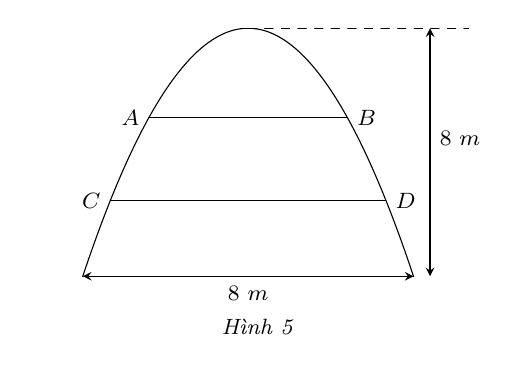
\begin{tikzpicture}[scale=0.7, font=\footnotesize, line join=round, line cap=round,>=stealth]
			\begin{scope}
				\clip (-4,-4.5) rectangle (4,0);
				\draw [smooth,domain=-5:4, samples=200] plot (\x, {-0.5*(\x)^2});
			\end{scope}
			\draw [<->] (3.3,0)--(3.3,-4.5);
			\node[right] at (3.3,-2){$8\,\,m$};
			\draw [<->] (-3,-4.5)--(3,-4.5);
			\node[below] at (0,-4.5){$8\,\,m$};
			\node[left] at (-1.8,-1.62){$A$};
			\node[right] at (1.8,-1.62){$B$};
			\node[left] at (-2.5,-3.125){$C$};
			\node[right] at (2.5,0-3.125){$D$};
			\draw [-] (-1.8,-1.62)--(1.8,-1.62);
			\draw [-] (-2.5,-3.125)--(2.5,0-3.125);
			\draw [dashed] (0,0)--(4,0);
			\node[below] at (current bounding box.south){\textit{Hình 5}};
		\end{tikzpicture}
	\end{center}
	% \shortans{ $1{,}26$                 }
	\loigiai{
	\immini{Gắn hệ trục tọa độ $Oxy$ vào cổng parabol như hình bên với trục $Oy$ trùng với đường đối xứng của parabol, gốc $O$ nằm ở đỉnh của parabol, đơn vị trên mỗi trục tính theo mét. Khi đó, phương trình parabol có dạng $y=ax^2$.\\
		Vì parabol đi qua điểm có toạ độ $(-4 ;-8)$ nên $a=-\dfrac{1}{2}$. Suy ra phương trình parabol là $y=-\dfrac{1}{2} x^2$.\\}{
		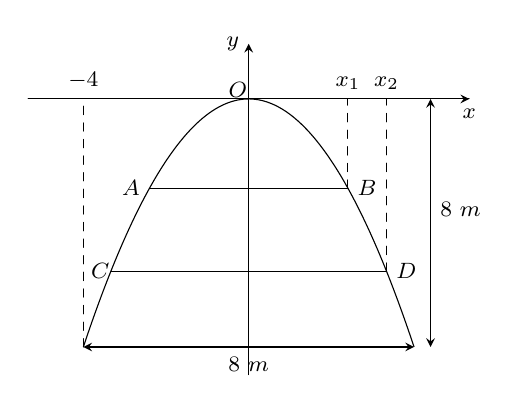
\begin{tikzpicture}[scale=0.7, font=\footnotesize, line join=round, line cap=round,>=stealth]
			\draw[->] (-4,0) --(4,0) node[below]{$x$};
			\draw[->] (0,-5) --(0,1) node[left]{$y$};
			\draw (0,0) node[above left=-3pt]{$O$};
			\begin{scope}
				\clip (-4,-4.5) rectangle (4,0);
				\draw [smooth,domain=-5:4, samples=200] plot (\x, {-0.5*(\x)^2});
			\end{scope}
			\draw [<->] (3.3,0)--(3.3,-4.5);
			\node[right] at (3.3,-2){$8\,\,m$};
			\draw [<->] (-3,-4.5)--(3,-4.5);
			\node[below] at (0,-4.5){$8\,\,m$};
			\node[left] at (-1.8,-1.62){$A$};
			\node[right] at (1.8,-1.62){$B$};
			\node[left=-3pt] at (-2.5,-3.125){$C$};
			\node[right] at (2.5,0-3.125){$D$};
			\draw [-] (-1.8,-1.62)--(1.8,-1.62);
			\draw [-] (-2.5,-3.125)--(2.5,0-3.125);
			\draw [dashed] (0,0)--(4,0) (1.8,-1.62)--(1.8,0) (2.5,0-3.125)--(2.5,0) (-3,-4.5)--(-3,0);
			\node[above] at (1.8,0){$x_1$};
			\node[above] at (2.5,0){$x_2$};
			\node[above] at (-3,0){$-4$};
		\end{tikzpicture}}
	Giả sử $B$ có hoành độ $x_1$,  $D$ có hoành độ $x_2$. Khi đó, phương trình đường thẳng $AB$ là $y=-\dfrac{1}{2} x_1^2$, phương trình đường thẳng $CD$ là $y=-\dfrac{1}{2} x_2^2$.\\
	Diện tích hình phẳng giới hạn bởi parabol và đường thẳng $AB$ là
	\[
		S_1=2\displaystyle\int\limits_0^{x_1}\left[-\dfrac 12x^2-\left(-\dfrac 12x_1^2\right)\right]\mathrm{\,d} x=\left.2\left(-\dfrac{x^3}6+\dfrac{x_1^2}2x\right)\right|_0^{x_1}=\dfrac 23x_1^3\,\,\left(\mathrm{m}^2\right).
	\]
	Diện tích hình phẳng giới hạn bởi parabol và đường thẳng $CD$ là
	\[
		S_2=2\displaystyle\int\limits_0^{x_2}\left[-\dfrac 12x^2-\left(-\dfrac 12x_2^2\right)\right]\mathrm{\,d} x=\left.2\left(-\dfrac{x^3}6+\dfrac{x_2^2}2x\right)\right|_0^{x_2}=\dfrac 23x_2^3\,\,\left(\mathrm{m}^2\right).
	\]
	Theo giả thiết, ta có  $S_2=2S_1\Leftrightarrow x_2^3=2x_1^3\Leftrightarrow\dfrac{x_2}{x_1}=\sqrt[3]2\approx 1{,}26$.\\
	Khi đó, $\dfrac{CD}{AB}=\dfrac{2x_2}{2x_1}\approx 1{,}26$.
	}
\end{ex}

\begin{ex}%[2H5V1-7]
	Từ mặt nước trong một bể nước, tại ba vị trí đôi một cách nhau $2$ m, người ta lần lượt thả dây dọi để quả dọi chạm đáy bể. Phần dây dọi (thẳng) nằm trong nước tại ba vị trí đó lần lượt có độ dài $4$ m; $4{,}4$ m; $4{,}8$ m. Biết đáy bể là phẳng. Hỏi đáy bể nghiêng so với mặt phẳng nằm ngang một góc bao nhiêu độ (làm tròn đến hàng phần chục)?
	% \shortans{$21{,}8$}
	\loigiai{
	Gọi ba vị trí trên mặt nước là $A$, $B$, $C$ thì tam giác $ABC$ là tam giác đều cạnh bằng $2$ m. Gọi dây dọi lần lượt là $AA'$, $BB'$, $CC'$ có độ dài lần lượt là $4$ m; $4{,}4$ m; $4{,}8$ m.\\
	Chọn hệ trục toạ độ $Oxyz$ sao cho $O$ là trung điểm của $BC$, tia $Ox$ chứa điểm $A$, tia $Oy$ chứa điểm $B$, tia $Oz$ đi qua trung điểm của $B'C'$ và đơn vị trên các trục là mét.\\
	Ta có $OB=OC=1$, $OA=\sqrt{3}$ $\Rightarrow$ $A'\left(\sqrt{3};0;4\right)$, $B'(0;1;4{,}4)$, $C'(0;-1;4{,}8)$.\\
	Khi đó, $\overrightarrow{A'B'}=\left(-\sqrt{3};1;0{,}4\right)$, $\overrightarrow{A'C'}=\left(-\sqrt{3};-1;0{,}8\right)$.\\
	Mặt phẳng $(A'B'C')$ có một véc-tơ pháp tuyến là $\overrightarrow{n}=\left[\overrightarrow{A'B'},\overrightarrow{A'C'}\right]=0{,}4\sqrt{3}\left(\sqrt{3};1;5\right)$.\\
	Mặt phẳng $(ABC)$ có một véc-tơ pháp tuyến là $\overrightarrow{k}=(0;0;1)$.\\
	Do đó, $\cos\big((ABC),(A'B'C')\big)=\left|\cos\left(\overrightarrow{n},\overrightarrow{k}\right)\right|=\dfrac{5}{\sqrt{29}}$. Góc cần tìm gần bằng $21{,}8^\circ$.
	}
\end{ex}
\Closesolutionfile{ans}


% \Closesolutionfile{ansbook}
% \HetDe
% \label{De4}
% %
% \cleardoublepage
% \setcounter{page}{1}
% \rfoot{Trang \thepage/\pageref{DA4} - Đáp án trắc nghiệm Mã đề 4}
% \begin{center}
% 	\bfseries ĐÁP ÁN TRẮC NGHIỆM MÃ ĐỀ 4
% \end{center}

% \inputansbox{10}{ans/ansDe4-TN1}
% \inputansbox[3]{2}{ans/ansDe4-TN2}
% \inputansbox{3}{ans/ansDe4-TN3}
% \label{DA4}
% %
